\documentclass[12pt]{article}

% Packages
\usepackage[utf8]{inputenc}
\usepackage[english]{babel}
\usepackage[top=3cm,bottom=3cm,left=3cm,right=3cm,bindingoffset=0mm]{geometry}
\usepackage{amssymb}
\usepackage{amsmath}
\usepackage{tikz}
\usepackage{graphicx}
\usepackage{comment}
\usepackage{rotating}
\usepackage{float}
\usepackage{natbib}
\usepackage{amsthm}
\usepackage{bbm}
\usepackage{thmtools,thm-restate}
\usepackage{hyperref}
%\usepackage{extsizes}
\usepackage[font=footnotesize,labelfont=bf]{caption}

% New Options
\newtheorem{prop}{Proposition}
\newtheorem{definition}{Definition}[section]
\newtheorem*{remark}{Remark}
\newtheorem{lemma}{Lemma}
\declaretheorem{proposition}
\linespread{1.3}
\raggedbottom
\font\reali=msbm10 at 12pt

% New Commands
\newcommand{\real}{\hbox{\reali R}}
\newcommand{\realp}{\hbox{\reali R}_{\scriptscriptstyle +}}
\newcommand{\realpp}{\hbox{\reali R}_{\scriptscriptstyle ++}}
\newcommand{\R}{\mathbb{R}}
\DeclareMathOperator{\E}{\mathbb{E}}

\title{ICT and Future Productivity:\\Evidence and Theory of a GPT\thanks{Correspondence: Department of Economics, Boston College, 140 Commonwealth Avenue, Chestnut Hill, MA 02467. Email: brianti@bc.edu (Marco Brianti) and gati@bc.edu (Laura G\'ati).}}
\author{Marco Brianti \\ {\small Boston College} \and Laura G\'ati \\ {\small Boston College}}
\date{\today}


\begin{document}



\maketitle

\

\

\
%%%%%%%%%%%%%%%%%%%%             ABSTRACT           %%%%%%%%%%%%%%%%%% 
\small{
\abstract{Information and Communication Technology (ICT) is able to explain accelerations in productivity in sectors that are ICT users. We employ Structural VARs to investigate the effects of ICT supply shocks on Total Factor Productivity (TFP) and other macroeconomic variables. In response to this sector-specific supply shock, relative prices of ICT goods and services immediately fall, ICT investment rises on impact, and TFP displays a significant delayed and persistent increase. Taking up the view of theories of ICT as a general-purpose technology, we analyze a two-sector general equilibrium model in order to rationalize previous results and estimate spillovers from the stock of ICT via impulse-response matching. We conclude that ICT accumulation is able to enhance productivity through a positive spillover effect which takes into account the overall level of diffusion of ICT capital in the economy.}
}
\newpage



\newpage
%%%%%%%%%%%%%%%%%%%%               INTRODUCTION                 %%%%%%%%%%%%%%%%%% 
\section{Introduction}

Although there is large consensus on the importance of productivity as a driver of economic performance, there is less agreement on the underlying sources of productivity growth. For several years most of the business-cycle literature purposely decided to avoid such a question by proxying movements in productivity as exogenous shocks.\footnote{\cite{kydland1982time} and \cite{long1983real} are among the first papers which consider productivity shocks on general equilibrium models.} However, the robust empirical evidence of the slowdown in productivity right before the Great Recession is urging the literature to take a step back and devote more attention on the drivers of medium-term productivity growth.\footnote{See \cite{cette2016pre} and \cite{byrne2016does} among others.}

Along with \cite{comin2006medium}, some theoretical contributions rationalize endogenous productivity dynamics by incorporating features of endogenous growth models into standard models of business cycles. Following \cite{romer1990endogenous}, most of these papers augment final-good production functions with an expanding composite of intermediate goods produced by the Research \& Development (R\&D) sector in order to allow for an endogenous rate of adoption of new technologies.\footnote{\cite{bianchi2014growth}, \cite{anzoategui2016endogenous}, and \cite{moran2017innovation} use similar techniques to endogenize growth. In particular, \cite{bianchi2014growth} augment a DSGE  model using a quality ladders model in the vein of \cite{grossman1991quality}. Moreover, \cite{anzoategui2016endogenous} and \cite{moran2017innovation}, similarly to \cite{comin2006medium}, use a model of expanding variety in the vein of \cite{romer1990endogenous}.} Guided by the prediction of such theoretical work that R\&D developments matter for growth, other papers attempt to provide empirical evidence of a slowdown in the productivity of the R\&D sector. Specifically, they show that although research effort keeps rising, the rate of new ideas and discoveries is slowing down.\footnote{\cite{jones2009burden} and \cite{bloom2017ideas} are two important contributions that highlight these facts.}

Motivated by this wave of research, this paper follows a different path and argues that Information and Communication Technology (hereafter ICT) plays an important role in driving medium-term productivity in sectors that are ICT users. Our contribution is twofold. First, we provide robust empirical evidence to show that current rises in ICT investment explains significant and persistent increases in future Total Factor Productivity (hereafter TFP). Second, we analyze a standard theoretical framework in order to both motivate and rationalize our empirical results. 

In the empirical section, we identify technological shocks specific to the ICT sector in a Structural VAR context.\footnote{An interesting paper related to our empirical work is \cite{jafari2012impact}. The authors identify ICT shocks as a potential driver of the Iranian business cycle using a completely different identification strategy and obtaining qualitatively different results.} In order to have a reliable identification procedure our multivariate system needs to include three key variables: TFP, ICT investment (hereafter ICTI), and relative prices (hereafter RP). ICTI is defined as the total expenditure in equipment and computer software meant to be used in production for more than an year. Thus, an increase in ICTI is ICT capital deepening. RP is the ratio between the price of the ICT good and the price level in the overall economy. We use two identifying restrictions in order to back out an ICT technology shock. First, we expect it to be orthogonal to the current productivity of all the other sectors. Since the share of the ICT sector accounts for a negligible part in the whole economy, ICT shocks should have an approximately zero effect on TFP on impact. Thus, our first restriction will be a zero-impact restriction on TFP after an ICT shock. Moreover, following \cite{greenwood1997long} and \cite{fisher2006dynamic}, we rely on RP and ICTI because we expect that a sectoral technology shock should decrease its relative prices and enhance expenditure in the underlying sector. For theoretical reasons discussed in more detail below, we do not impose any restriction on RP; instead, we let the ICT shock maximize the impact response of ICTI.\footnote{However, as suggested by both \cite{greenwood2000role} and \cite{basu2010sector}, we are aware that conditioning our identifying restrictions only on the direction of RP does not properly measure for technological changes between sectors. This is the main reason why we never impose the direction of RP as an direct identifying condition.} In response to this shock, ICTI rises on impact and remains significant for several quarters. RP persistently and significantly declines for more than two years, suggesting that we are indeed identifying the correct sectoral shock. Our main result is that TFP, restricted not to respond on impact, rises after few quarters and remains significant and stable for at least 5 years, despite the tiny size of the ICT sector relative to the economy. 

Although our results are robust over different specifications, an important critique to our empirical strategy is reverse causality coming from news on future TFP. As suggested by the news-shock literature, the positive reaction of ICTI on impact may be triggered by signals related future increases in TFP and not to contemporaneous ICT technological improvements. In other words, our identification strategy may confound our shock of interest with a news shock which contemporaneously enhances investment in ICT capital goods. We address this issue by providing a series of alternative identification strategies which we show deliver the same time series of ICT innovations as our initial specification. The heart of these robustness checks is sequential identification of news and ICT shocks: we firstly identify a news shock in the spirit of \cite{barsky2011news}, and subsequently we identify our sectoral ICT shock using the previous identification strategy. Encouragingly, controlling for signals regarding future movements in TFP does not affect our results. We view this as strengthening our statement relating movements in current ICT technology to future TFP. 


In order to formally explain which mechanism links current ICT to future TFP, we analyze a two-sector DSGE model which allows ICT to be the general purpose technology (hereafter GPT) of the whole economy. There are two main justifications for interpreting ICT as a GPT. On the one hand, there is a vast literature that makes a case for the general-purpose nature of ICT capital.\footnote{See for example \cite{oliner2000resurgence} and \cite{stiroh2002information} amongst others.} On the other hand, the small size of ICT sector share both in overall investment and overall output makes our results of a strong and persistent TFP increase after an ICT shock hard to interpret in absence of an additional force such as an externality coming from the general-purpose property of ICT capital.

In our model, both sectoral production functions are fed with three inputs: (i) labor, supplied by households, (ii) hard capital, produced by the final sector, and (iii) ICT capital, produced by the ICT sector. As explained by both \cite{basu2003case} and \cite{basu2007information}, a GPT should be able to enhance accelerations in productivity in sectors that are users of the underlying technology. We then interpret ICT as the GPT of the last 30 years of the U.S. economy assuming that exogenous technological changes in the ICT sector are able to affect economy-wide productivity above the direct effect coming from the technology increase itself.\footnote{A clarification is in place here. In a two-sector model, the overall residual productivity is a convolution of the two exogenous productivities. Thus sectoral productivity changes trivially show up in overall productivity. Our assumption of ICT capital being a GPT means that overall productivity responds more to an ICT-sector-specific technology shock than warranted by this shock directly. We address this question in detail in the main text in Section \ref{section:empirics}.} In particular, when an ICT technology shock arrives, both sectors accumulate ICT capital since it is easier to produce and cheaper to buy. This ICT capital deepening consequently enhances the productivity of both sectors by means of a spillover. 

Since the purpose of ICT capital is to improve information sharing, the quality and speed of communication mainly depends on the diffusion of these technologies among agents. As a simple example, owning a mobile phone enables one to contact another person instantaneously only if the other person is also endowed with the same technology. As a result, the effectiveness of ICT capital is intrinsically related to its own diffusion. We rationalize this line of thought augmenting the production function of each sector with a spillover effect driven by the diffusion of ICT capital. Consistently with the GPT literature above and our empirical results, the accumulation of ICT capital is a slow process and the benefits of an ICT technology shock show up in the production functions of ICT-users with lags.\footnote{Notice that differently to \cite{basu2003case} and \cite{basu2007information}, we interpret the general-purpose nature of ICT in the spirit of an endogenous growth model.}

As a last step, we use both our empirical and theoretical results to estimate the key parameters of the model via impulse-response function matching to an ICT technology shock. The key parameters within this set are (i) the elasticity of productivity to ICT capital diffusion, namely the parameter which governs the spillover effect, and (ii) the standard deviation and (iii) persistence of ICT technology shocks. Results consistently point out a positive spillover effect of ICT capital deepening on TFP suggesting that the assumptions made in the theoretical model are supported by our empirical results. We confirm that ICT is a general-purpose technology which enhance productivity of ICT capital users through a spillover effect related to its own diffusion.

\begin{comment}
Our paper is mainly related to three strands of literature. First of all, we link to the literature that investigates the recent slowdown in TFP growth. Our project is motivated by papers such as \cite{oliner2007explaining}, \cite{jorgenson2008retrospective}, \cite{byrne2016does}, \cite{cette2016pre}, and \cite{fernald2017disappointing} who document that the slowdown in TFP growth occurred before the recession implying that the financial crisis per se cannot be its cause.\footnote{In particular, in line with our results, also \cite{fernald2017disappointing} conclude that the pause in the information technology revolution is the main candidate explanation.} Secondly, our project is related to the literature that investigate the effects of investment-specific technology shocks in a multi-sector economy. In particular, throughout the paper our main references will be \cite{greenwood1997long}, \cite{oulton2007investment}, and \cite{fisher2006dynamic}. However, both the empirical exercise and the theoretical model are strictly related to \cite{greenwood2000role}, \cite{basu2010sector}, and \cite{justiniano2011investment}. Finally, this paper is also related to papers that argue that information and communication technology is the current general-purpose technology. Main references will be bresnan, and \cite{basu2007information}.
\end{comment}

The paper is structured as follows. We present empirical results and main robustness checks in Section \ref{section:empirics}. We then present and analyze the two-sector DSGE model in Section \ref{section:theory}. We estimate via impulse-response matching key parameters of the model and run a series of related experiment in Section \ref{section:experiments}. Concluding remarks, caveats and prospective future research are discussed in Section \ref{section:conclusions}.



%%%%%%%%%%%%%%%%%%%%%%            EMPIRICS                     %%%%%%%%%%%%%%%%%%%
\section{Empirics}\label{section:empirics}

In this section we present our main empirical set of results. Our attempt is to properly identify technological shocks which are only specific to the ICT sector in a Structural VAR context and analyze their impact on key macroeconomic variables.

\subsection{Main Specification}\label{section:mainSpec}

In this section we present our main specification where we impose minimal discipline on the identification strategy. It turns out that the set of results presented here are consistent with different robustness checks.

\subsubsection{Data}

Our first-step specification is the following 5-variable VAR 
\begin{equation}\label{eq:mainSpecification}
\begin{pmatrix}
TFP_t \\ 
ICTI_t \\
GDP_t \\
C_t \\
RP_t \\
\end{pmatrix} = B(L) \begin{pmatrix}
TFP_{t-1} \\ 
ICTI_{t-1} \\
GDP_{t-1} \\
C_{t-1} \\
RP_{t-1} \\
\end{pmatrix} + i_t
\end{equation}
where $TFP_t$ is the log-level of Fernald total factor productivity at time $t$, $ICTI_{t}$ is the log-level of real information and communication technology investment at time $t$,\footnote{Notice that $ICTI_t$ is defined as the total expenditure at time $t$ in equipment and computer software meant to be used in production for more than an year.} $GDP_t$ is the log-level of real gross domestic product at time $t$, $C_t$ is the log-level of real consumption at time $t$, and $RP_t$ is the log-deviation of ratio between prices of ICT goods and services and the consumer price index (CPI).\footnote{Except for $RP_t$ that is not cointegrated with the remaining variables, we opt for estimating the VAR in levels since it produces consistent estimates of the impulse responses and is robust to cointegration of unknown forms. In particular, as suggested by \cite{hamilton1994time} when there is uncertainty regarding the nature of common trends, estimating the system in levels is considered the conservative approach. In any case our results are very similar when estimating a vector error correction model (VECM).} All the variables have a quarterly frequency from 1989:Q1 to 2017:Q1 and refer to the U.S. economy. $B(L)$ is a ($5\times 5$) matrix of lag-operator functions of the same order. Following the Bayesian Information Criterion (BIC), the lag operator functions is one which implies that we regress variables at time $t$ with their own lagged values at $t-1$.\footnote{The Hannan-Quinn Criterion (HQ) suggests to use two lags. Results remains consistent following this second criterion.} Finally, $i_t$ is a ($5 \times 1$) vector of correlated innovations where $\Sigma = i'_t i_t$.

\subsubsection{Empirical Strategy}


Our simplest identification strategy implies that an ICT-investment technological shock (hereafter ICT shock) has no impact effect on TFP and maximal impact effect on ICTI. We justify these assumptions with both empirical and theoretical argument. First of all, using data released on April, 2018 by the Bureau of Economic Analysis (BEA) the real value added of the information sector on real GDP is slightly below $5$\% for the underlying quarter. Thus, since the share of this sector accounts for a negligible part in the whole economy, we assume that an ICT shock is orthogonal to current TFP. In addition, in line with theoretical results firstly presented by \cite{greenwood1997long}, we expect that an ICT shock should enhance sector-specific investment since ICT goods are now easier to produce and cheaper to buy. As a result, we expect an ICT shock to have a maximal impact effect on ICTI. 

Following a similar notation of \cite{barsky2011news}, we implement our identification strategy as follows. Let $y_t$ be the $(5 \times 1)$ vector of observables of length $T$ presented above. Once can form the reduced form moving average representation:
$$
y_t = \bar{B}(L)y_{t} + i_t \ \ \Rightarrow \ \ y_t = A(L)i_t
$$
where $A(L) = [I - \bar{B}(L)]^{-1}$ and $\bar{B}(L)$ has no constant terms. Assume now there exists a linear combination that maps innovations $i_t$ to structural shocks $s_t$:
$$
s_t = A_0 i_t
$$
This entails the structural moving average representation:
$$
y_t = C(L)i_t
$$
where $C(L) = A(L) A_0$ and $i_t = A_0^{-1} s_t$. The impact matrix $A_0$ must be such that $\Sigma = A_0 A_0'$. Notice that $A_0$ is not unique since for any $D$ such that $DD' = I$, $\tilde{A}_0 = A_0 D$ satisfies $\Sigma = \tilde{A}_0 \tilde{A}_0'$. 

The matrix of impact responses to all shocks is:
$$
\Omega = \tilde{A}_0 D
$$
and is specifically formed by the following elements,
$$
\Omega_{i,j} = e_i' \tilde{A}_0 D e_j
$$
where $e_k$ is a selection column vector of the same dimension of $\tilde{A}_0$ with $1$ in the $k$th element and zero elsewhere. In particular, notice that $e_j$ is selecting a specific column of $D$, which will be denoted by $\gamma_j$. As a result, $\tilde{A}_0\gamma_j$ denotes the vector of impact responses of all the variable to shock $j$.

Let observe from System \ref{eq:mainSpecification} that $TFP_t$ is ordered first and $ICTI_t$ second. In order to implement our identification strategy, we need to mathematically solve the following problem:
\begin{equation}\label{eq:mainObjective}
\max_{\gamma_j} \Omega_{2,j} = e_2' \tilde{A}_0 \gamma_j
\end{equation}
subject to
\begin{equation}\label{eq:mainZeroTFP}
\Omega_{1,j} = e_1' \tilde{A}_0 \gamma_j = 0, \ \ \text{and}
\end{equation}
\begin{equation}\label{eq:mainOrtho}
\gamma_j' \gamma_j = 1
\end{equation}
where $j$ represents the arbitrary position of the ICT shock. Then, in order to ensure that this identification belongs to the space of possible orthogonalizations of $\Sigma$, the problem is denoted in terms of choosing $\gamma_j$ conditional on any orthogonalization, $\tilde{A}_0$. Objective function \ref{eq:mainObjective} imposes that an ICT shock as a maximal impact effect on ICT investment. Constraint \ref{eq:mainZeroTFP} orthogonalizes current TFP to ICT shocks and Constraint \ref{eq:mainOrtho} satisfies the condition that $\gamma_j$ is derived from an orthogonal matrix $D$.  

\subsubsection{Main Set of Results}

Appendix \ref{section:mainSetResults} shows the estimated impulse responses of System \ref{eq:mainSpecification} to the identified ICT shock. The shaded gray areas are the $90$\% and $95$\% confidence bands from 2000 bias-corrected bootstrap procedure of \cite{kilian1998small}. In particular, Figure \ref{fig:TFP_main} shows impulse response of TFP to an ICT shock. TFP takes around $4$ quarters before displaying a positive and significant effect and reaches its peak of $1.2$\% after $24$ quarters. In Figure \ref{fig:ICT_main}, real ICT investment has a large and positive impact response of almost $2$\% that gets even larger after a quarter. Then, it slowly starts to decay remaining significant for more than $40$ quarters. In Figures \ref{fig:GDP_main} and \ref{fig:C_main}, we present responses of real GDP and real consumption, respectively. Real GDP has a significant impact response of $0.3$\% and reaches its peak of almost $0.5$\% approximately at the same time of TFP. Similarly, real consumption has an impact effect of $0.2$\% with a delayed peak of $0.5$\%. Finally, in Figure \ref{fig:RP_main}, relative prices has a significant and negative impact response of $0.4$\% and remain persistently below their own steady state value for almost $9$ years.

In addition, Table \ref{table:vardec} in Appendix \ref{section:vardec} presents forecast error variance of each variable on impact, and after one-, two-, four-, six-, and ten-year horizon. In line with impulse responses, ICT shocks, which are orthogonal to current productivity, explain a third of TFP fluctuations over ten-year horizon. On the other hand, ICT shocks drive almost the whole variation in ICT investment on impact but this effect tends to decay over time getting below the $50$\% after 10 years. Interestingly, both output and consumption has a remarkable reaction on impact: $26$\% and $19$\%, respectively. Moreover, this effect tends to increase reaching $40$\% in both cases over the maximal horizon. Finally, ICT shocks do not have a remarkable effect on relative prices. The fraction of fluctuations explained on impact is only $6$\% with a peak of $14$\% between four and six years.

\subsection{Controlling for News Shocks}

In this section, we show a set of robustness checks aimed to show that our previous results are not driven by future signals regarding exogenous productivity. Although our results are robust when we purposely change the main specification presented in Subsection \ref{section:mainSpec}, an important critique to our empirical strategy is reverse causality coming from news on future TFP. As suggested by the news-shock literature, the positive reaction of ICTI on impact may be triggered by signals related future increases in productivity and not to a contemporaneous ICT shock. In other words, our identification strategy may confound our shock of interest with a news shock which contemporaneously enhances investment in ICT capital goods. We address this issue by providing two main alternative identification strategies which we show deliver the same time series of ICT shocks as our initial specification. Firstly, we test if our result is robust once removed all the forward looking variables which fluctuations may be unrelated to sector-specific technological changes: consumption and output. Technically speaking, consumption and output may granger-cause future TFP for reasons which are orthogonal to ICT shocks. For example, the forward-looking nature of consumption may provide to the VAR unnecessary information regarding future changes in TFP not related to an ICT shock which our identification strategy is not able to filter it out. Secondly, we apply a sequential identification where we firstly identify a news shock in the spirit of \cite{barsky2011news}, and subsequently we identify our sectoral ICT shock using the previous identification strategy. This second strategy has the specific purpose of filtering out all the current movements in forward-looking variables related to future fluctuations of TFP which are not related to current ICT shocks.

Encouragingly, controlling for signals regarding future movements in productivity does not affect our identified ICT shocks suggesting a causal relation which goes from current ICT investment to future TFP.

\subsubsection{Removing Forward-Looking Variables}

Three-variables one lag, just show the structural shocks and their correlation. Responses very similar.

\subsubsection{Sequential Identification Strategy}



%%%%%%%%%%%%%%%%%%%%               MODEL                 %%%%%%%%%%%%%%%%%% 
\section{Model}\label{section:theory}


%%%%%%%%%%%%%%%%%%%%               MODEL                 %%%%%%%%%%%%%%%%%% 
\section{Experiments}\label{section:experiments}




%%%%%%%%%%%%%%%%%%%%               CONCLUSION                 %%%%%%%%%%%%%%%%%% 
\section{Conclusion}\label{section:conclusions}
hjklbhjkl

\bibliographystyle{chicago}
\bibliography{literature}

 %%%%%%%%%%%%%%%%%%           BIBLIOGRAPHY            %%%%%%%%%%%%%%%%%% 

\newpage

 %%%%%%%%%%%%%%%%%%           Appendices            %%%%%%%%%%%%%%%%%% 

\appendix 

\section{Main Set of Results}\label{section:mainSetResults}

	\begin{figure}[h!]
		\begin{center}
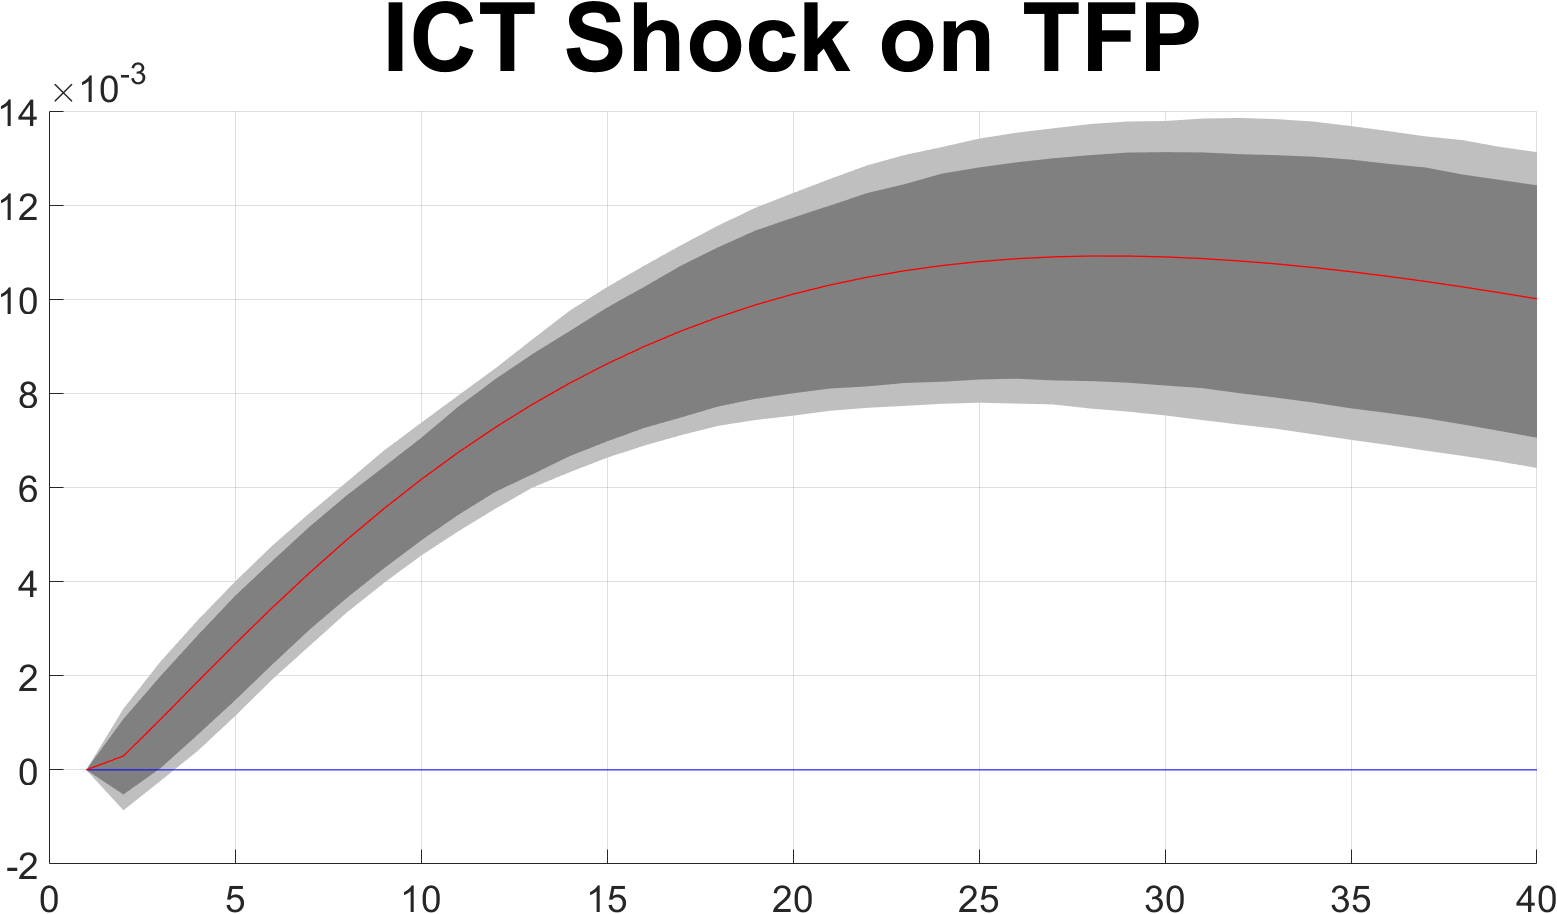
\includegraphics[scale=0.35]{MainFigures/fig_ICT_Shock_on_TFP_empirical_noH}
		\caption{Empirical impulse response of TFP to an ICT shock. The red solid lines are the estimated impulse responses to our ICT shock. The shaded dark gray area and the shaded light gray area are the $90$\% and $95$\% confidence intervals, respectively, from 2000 bias-corrected bootstrap replications of the reduced-form VAR. The horizontal axes refer to forecast horizon and the units of the vertical axes are percentage deviations.}
		\label{fig:TFP_main}
	\end{center}
\end{figure}

\newpage




	\begin{figure}[h!]
		\begin{center}
		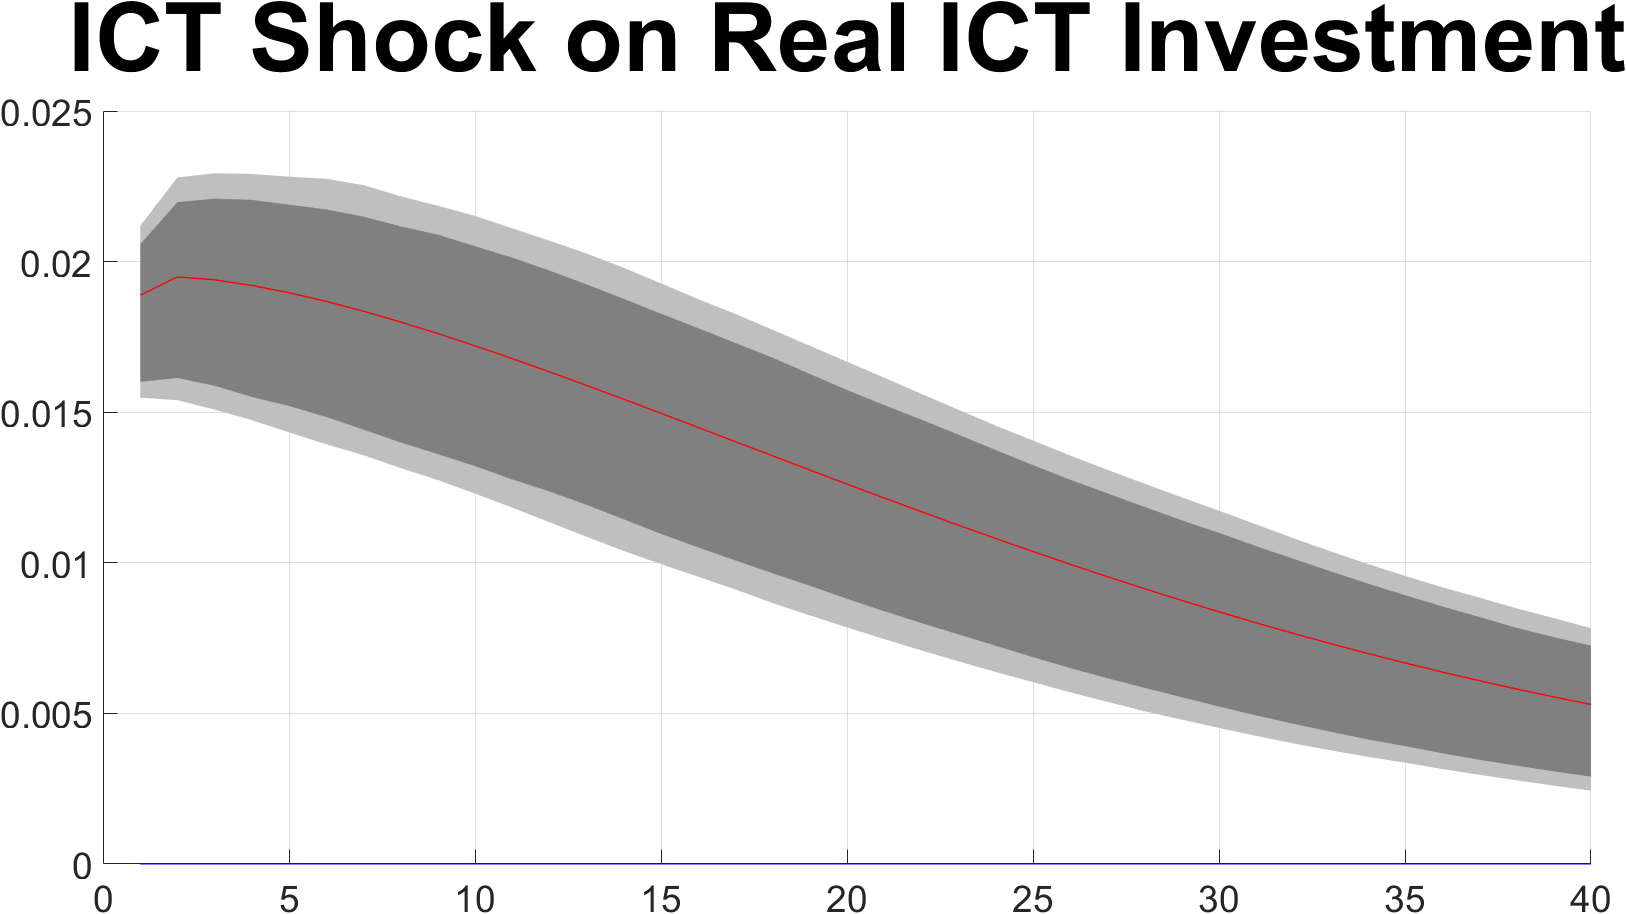
\includegraphics[scale=0.35]{MainFigures/fig_ICT_Shock_on_Real_ICT_Investment_empirical_noH}
		\caption{Empirical impulse response of real ICT investment to an ICT shock. The red solid lines are the estimated impulse responses to our ICT shock. The shaded dark gray area and the shaded light gray area are the $90$\% and $95$\% confidence intervals, respectively, from 2000 bias-corrected bootstrap replications of the reduced-form VAR. The horizontal axes refer to forecast horizon and the units of the vertical axes are percentage deviations.}
		\label{fig:ICT_main}
	\end{center} 
	\end{figure}

\newpage


	\begin{figure}[h!]
	\begin{center}
		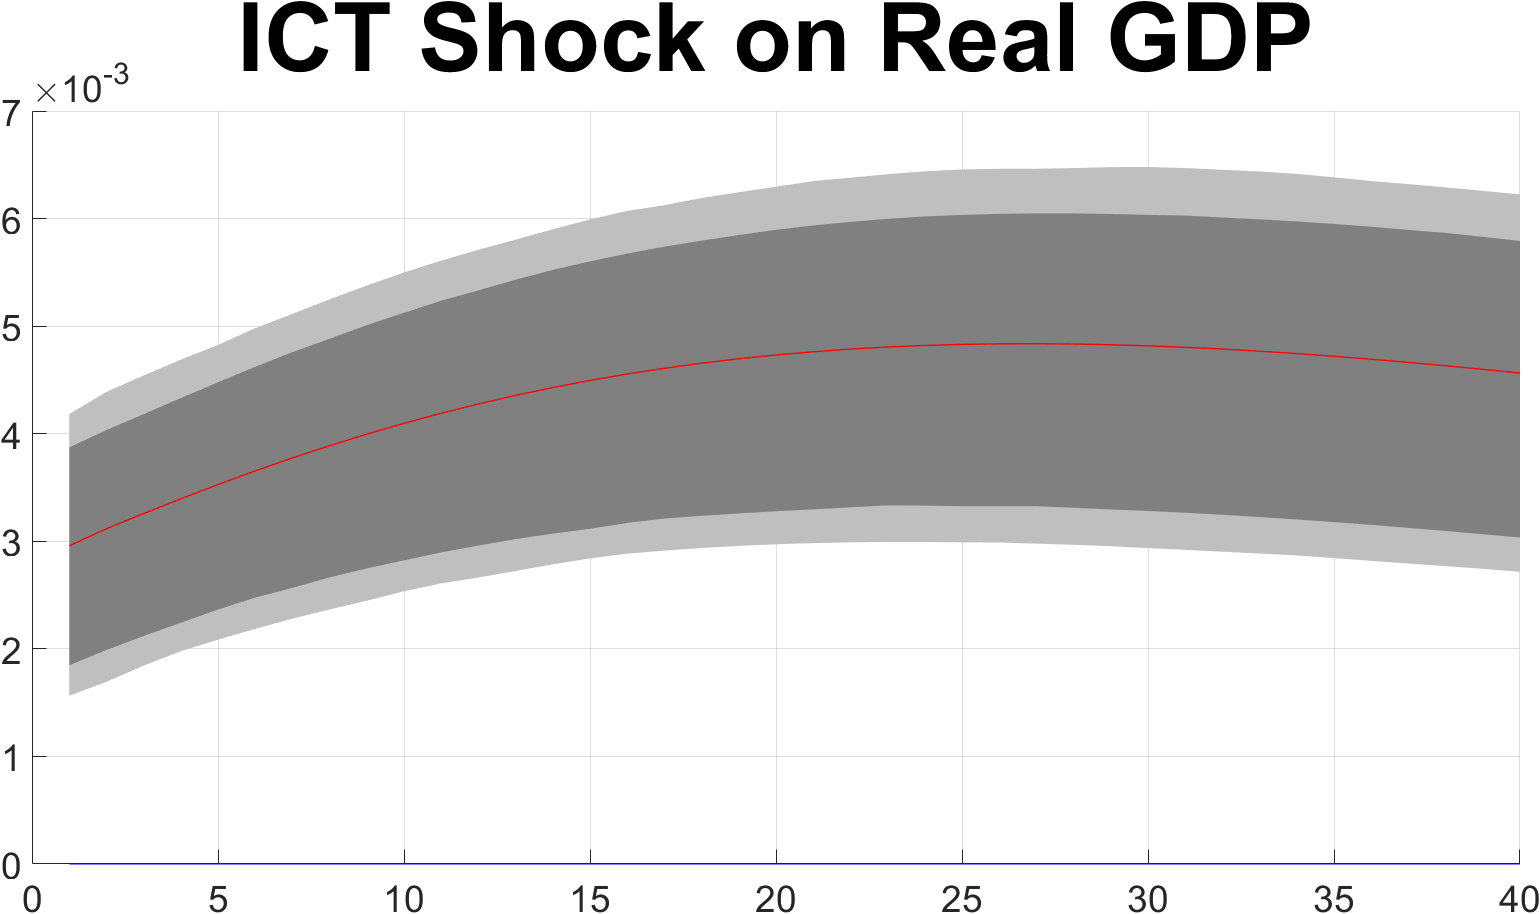
\includegraphics[scale=0.35]{MainFigures/fig_ICT_Shock_on_Real_GDP_empirical_noH}
		\caption{Empirical impulse response of real Gross Domestic Product to an ICT shock. The red solid lines are the estimated impulse responses to our ICT shock. The shaded dark gray area and the shaded light gray area are the $90$\% and $95$\% confidence intervals, respectively, from 2000 bias-corrected bootstrap replications of the reduced-form VAR. The horizontal axes refer to forecast horizon and the units of the vertical axes are percentage deviations.}
		\label{fig:GDP_main}
	\end{center} 
\end{figure}

\newpage


	\begin{figure}[h!]
	\begin{center}
		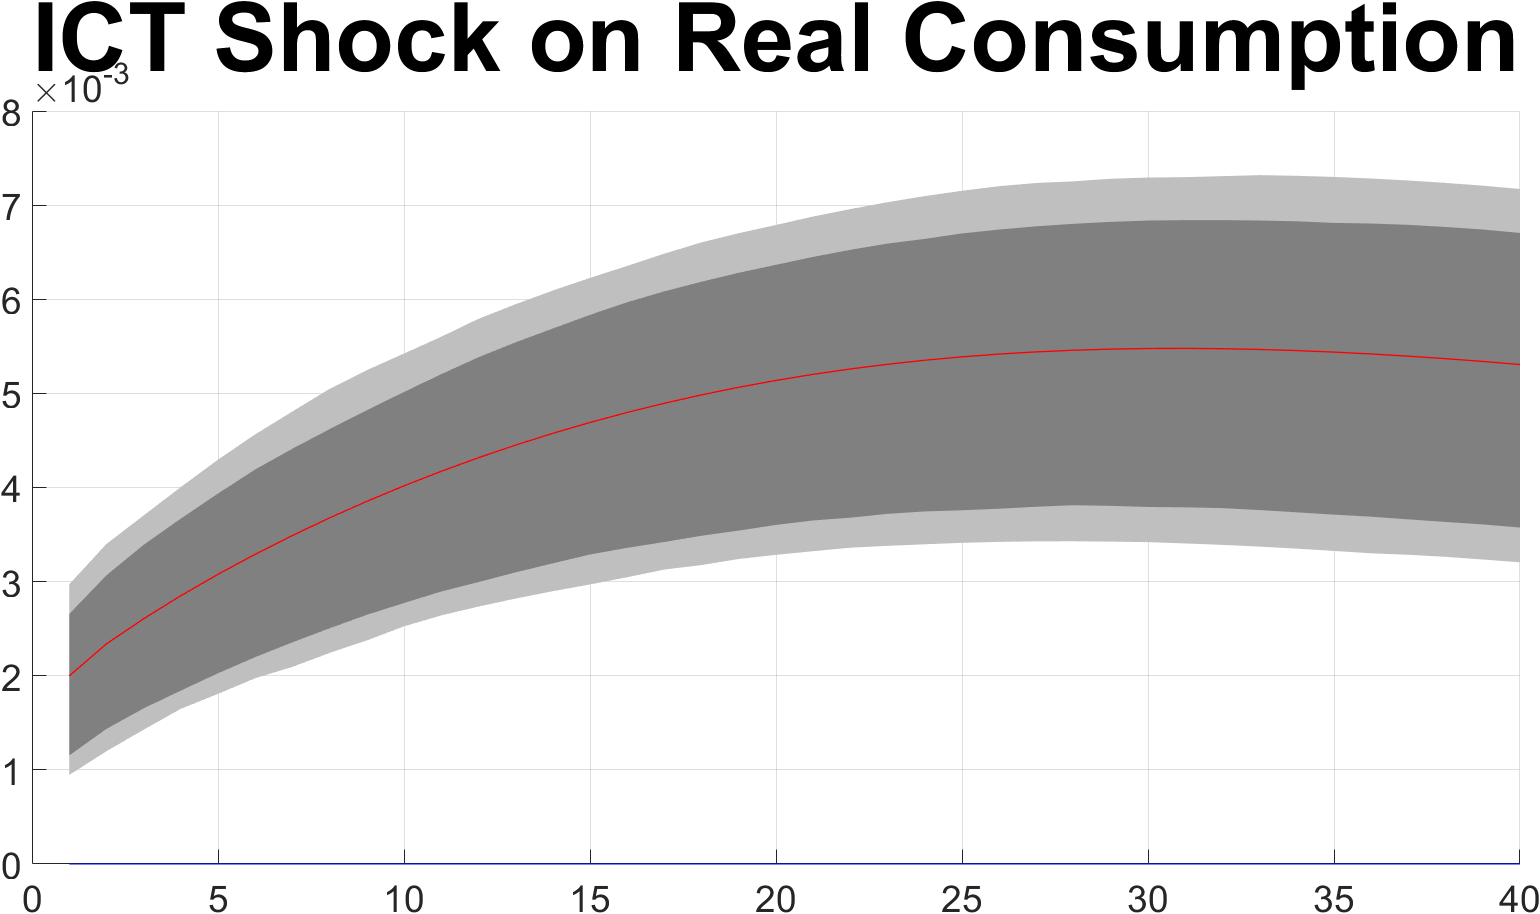
\includegraphics[scale=0.35]{MainFigures/fig_ICT_Shock_on_Real_Consumption_empirical_noH}
		\caption{Empirical impulse response of real consumption to an ICT shock. The red solid lines are the estimated impulse responses to our ICT shock. The shaded dark gray area and the shaded light gray area are the $90$\% and $95$\% confidence intervals, respectively, from 2000 bias-corrected bootstrap replications of the reduced-form VAR. The horizontal axes refer to forecast horizon and the units of the vertical axes are percentage deviations.}
		\label{fig:C_main}
	\end{center} 
\end{figure}

\newpage


	\begin{figure}[h!]
	\begin{center}
		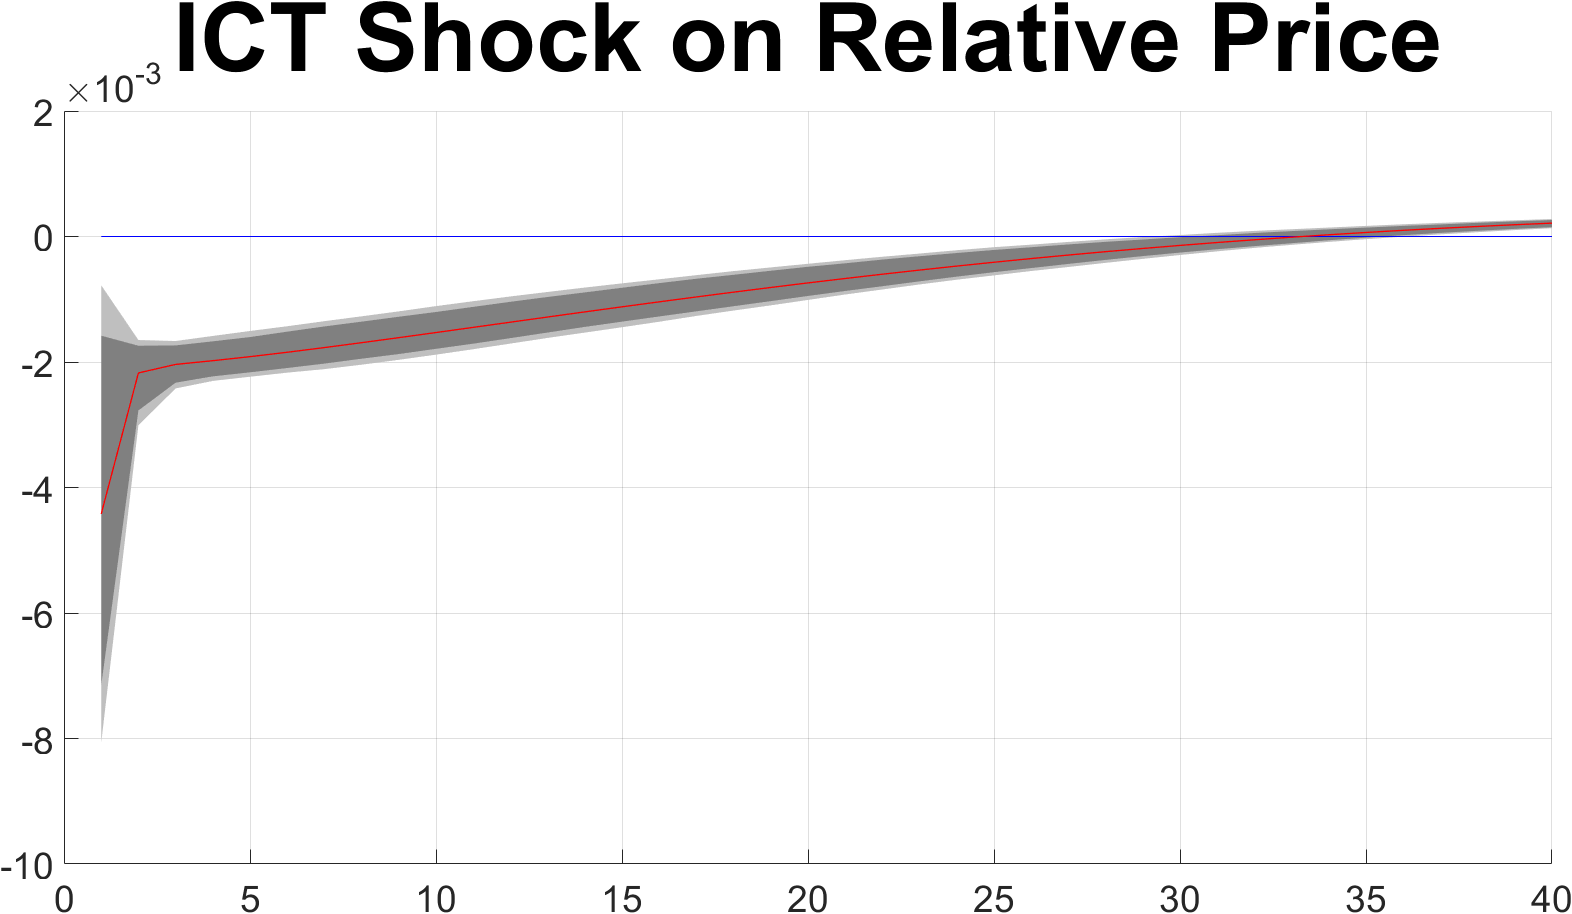
\includegraphics[scale=0.35]{MainFigures/fig_ICT_Shock_on_Relative_Price_empirical_noH}
		\caption{Empirical impulse response of relative price to an ICT shock. The red solid lines are the estimated impulse responses to our ICT shock. The shaded dark gray area and the shaded light gray area are the $90$\% and $95$\% confidence intervals, respectively, from 2000 bias-corrected bootstrap replications of the reduced-form VAR. The horizontal axes refer to forecast horizon and the units of the vertical axes are percentage deviations.}
		\label{fig:RP_main}
	\end{center} 
\end{figure}




\newpage

 
 
 \section{Variance Decomposition}\label{section:vardec}

 
 
 	\begin{table}[h!]
 		\begin{center}
 \begin{tabular}{lcccccccccc}
\hline
 	& $h = 1$ & $h = 4$ & $h = 8$ & $h = 16$ & $h = 24$ & $h = 40$ \\
 	\hline
TFP &  0       &  0.0023  &  0.0194 &   0.1088 &   0.2273  &  0.3382 \\
ICT Investment &  0.9997  &  0.9038  &  0.7964 &   0.6320 &   0.5310  &  0.4371 \\
Real GDP &  0.2620  &  0.3061  &  0.3486 &   0.3936 &   0.4046  &  0.3881 \\
Real Consumption &  0.1952  &  0.2638  &  0.3219 &   0.3931 &   0.4188  &  0.4064 \\
Relative Prices &  0.0618  &  0.0967  &  0.1276 &   0.1511 &   0.1516  &  0.1467 \\	
\hline
 	\end{tabular}
  		\caption{The letter $h$ denotes the forecast horizon. The numbers refer to the fraction of the forecast error variance of each variable at various forecast horizons to the identified ICT shock}
  \label{table:vardec}
  \end{center}
 \end{table}

 
\end{document}


